% Packages & Document Configurations
\documentclass[twocolumn]{NobArticle}
\runninghead{Shortened Running Article Title}
%\footertext{\textit{Journal X} (2023) 12:684}
\usepackage{chemformula}
% Title
\title{Determination of Corrosion Rate of Different Metals by Tafel Plots}

% Authors
\author{
    Jhon Aponte\textsuperscript{1}, 
    Josue Moreira\textsuperscript{1} 
    and Diego Cedeno\textsuperscript{1}
}

% Affiliations
\date{
    \textsuperscript{\textbf{1}}
    School of Chemical and Engineering sciences 
}

% Abstract
\renewcommand{\maketitlehookd}{%
\begin{abstract}
This study investigates the electrochemical corrosion behavior of admiralty brass and steel electrodes through potentiodynamic polarization measurements and Tafel plot analysis in 0.5 M hydrochloric acid medium. The corrosion kinetics were evaluated using a three-electrode electrochemical cell configuration with titanium as counter electrode and Ag/AgCl (3 M KCl) as reference electrode. 

Open circuit potential measurements revealed initial values of \(-142.9 \, \text{mV}\) for brass and \(-441 \, \text{mV}\) for steel. Linear sweep voltammetry was conducted at a scan rate of \(1 \, \text{mV/s}\) within \(\pm 200 \, \text{mV}\) around the open circuit potential to construct Tafel plots and determine corrosion parameters through linear extrapolation methods. 

The brass electrode exhibited a corrosion current density of \(5.40 \times 10^{-6} \, \text{A/cm}^2\) and a corrosion potential of \(-0.258 \, \text{V}\), resulting in a corrosion penetration rate (CPR) of \(4.17 \times 10^{-5} \, \text{mm/year}\). The steel electrode showed a corrosion current density of \(8.87 \times 10^{-5} \, \text{A/cm}^2\) and a corrosion potential of \(-0.388 \, \text{V}\), yielding a CPR of \(8.23 \times 10^{-4} \, \text{mm/year}\). 

The anodic and cathodic Tafel slopes were determined through linear regression analysis of the polarization curves.
\medskip

\small{\textbf{Keywords:} Electrochemical corrosion, Tafel plots, potentiodynamic polarization, corrosion rate, admiralty brass, steel}
\end{abstract}
}

\begin{document}

\small
\maketitle

\section{Introduction}
Metallic corrosion represents one of the most significant phenomena in the degradation of materials, being a spontaneous electrochemical process that involves the oxidation of the metal in the presence of an oxidizing agent from the environment. This process results in the progressive loss of mechanical and structural properties, generating severe economic and safety consequences in industrial applications. The electrochemical mechanism of corrosion is based on the formation of microscopic galvanic cells on the metallic surface, where anodic reactions (metal oxidation) and cathodic reactions (reduction of the oxidizing agent) occur simultaneously. In the specific case of steel in acidic media, the reactions can be represented as:

\textbf{Anodic reaction:} Fe $\rightarrow$ Fe$^{2+}$ + 2e$^{-}$

\textbf{Cathodic reaction:} 2H$^{+}$ + 2e$^{-}$ $\rightarrow$ H$_2$

The rate of these processes is controlled by kinetic factors that can be studied through advanced electrochemical techniques. Among them, Tafel plots are a fundamental tool for the quantitative characterization of corrosion processes, allowing for the accurate determination of critical kinetic parameters such as the corrosion potential ($E_{\mathrm{corr}}$) and the corrosion current density ($j_{\mathrm{corr}}$)~ \cite{stern1957}.

This technique is based on the Tafel equation:



\[
\eta = \pm b \log \left(\frac{j}{j_0}\right)
\]



where $\eta$ is the overpotential, $b$ is the Tafel slope, $j$ is the current density, and $j_0$ is the exchange current density. The interpretation of Tafel plots involves identifying linear regions in the anodic and cathodic branches of the semilogarithmic potential vs. log(current density) curve. The extrapolation of these linear regions until their intersection directly provides the values of $E_{\text{corr}}$ and $j_{\text{corr}}$. This procedure, known as Tafel extrapolation, is widely recognized for its precision and reproducibility in corrosion evaluation, although it must be noted that in certain systems only one branch may exhibit a well-defined linear region due to passivation, diffusion, or other mechanistic effects.

The corrosion penetration rate (CPR) is calculated by applying Faraday’s law of electrolysis:



\[
\mathrm{CPR} = \frac{0.13 \times j_{\mathrm{corr}} \times \mathrm{E.W.}}{\rho}
\]



where E.W. is the equivalent weight of the metal (g/\text{equiv}), $\rho$ is the density (g/cm$^3$), and $j_{\mathrm{corr}}$ is expressed in $\mu$A/cm$^2$. This relationship allows the conversion of electrochemical data into practical corrosion rates expressed in units such as $\mathrm{mpy}$ (mils per year). The constant 0.13 results from a combination of Faraday’s constant and unit conversions, and it is valid only when the parameters are expressed in the specified units.

The Tafel plot technique finds extensive applications in evaluating the corrosion resistance of alloys, testing the efficiency of corrosion inhibitors, and characterizing protective coatings. In industrial practice, this methodology enables the prediction of the service life of metallic components and the optimization of cathodic protection strategies. Moreover, the application of linear sweep voltammetry to construct potentiodynamic polarization curves provides further insights into corrosion mechanisms, including the identification of passivation processes, pitting, and intergranular corrosion \cite{bard2001}.

\section{Experimental Section}

\subsection{Materials and Equipment}

The following materials and equipment were used for the electrochemical corrosion experiments:

\begin{itemize}
    \item Electrochemical cell
    \item Magnetic stirrer
    \item Crocodile clips
    \item Micrometer
    \item Electric wires
    \item Sandpaper (grit sizes: 500, 1000, and 1500)
    \item 500 mL beaker
    \item Washing bottle
    \item Working electrodes: admiralty brass and copper
    \item Counter electrode: titanium plate
    \item Reference electrode: Ag/AgCl (3 M KCl; \( E^\circ = 0.210 \) V vs. NHE)
    \item Potentiostat and galvanostat
\end{itemize}

\subsection{Reagents}

The chemical reagents used in the experiment included:

\begin{itemize}
    \item Hydrochloric acid (concentrated and diluted)
    \item Distilled water
    \item Acetone
    \item Ethanol
\end{itemize}

\subsection{Methods}

The experimental procedure was followed as outlined below.

\begin{figure}[ht!]
    \centering
    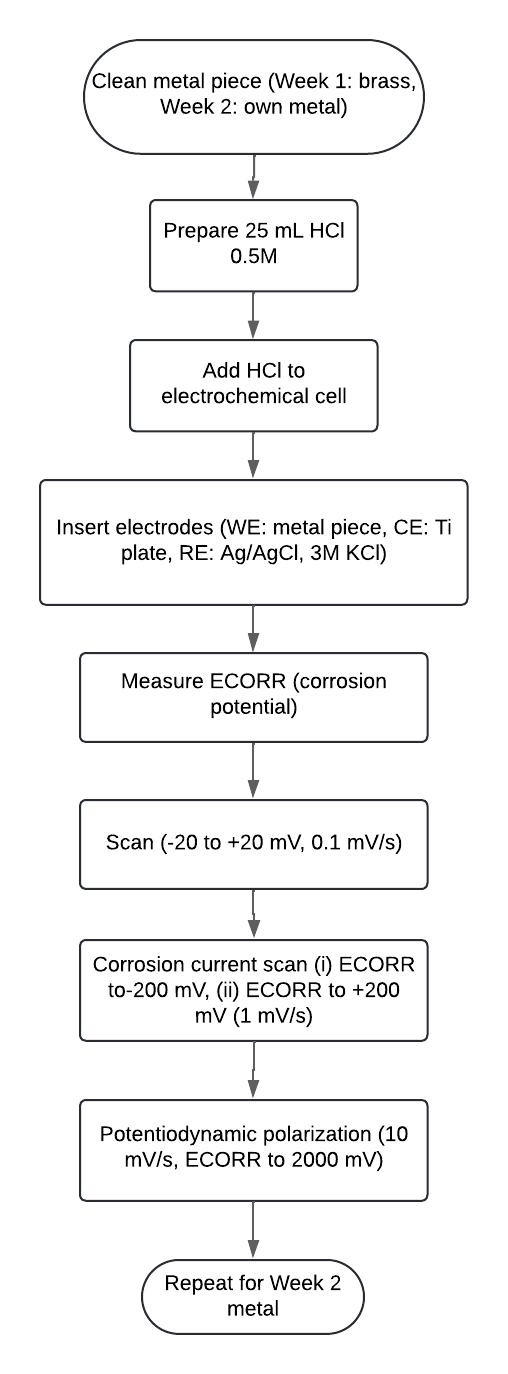
\includegraphics[width=0.50\columnwidth]{Figures/FLOWCHART 4.png}
    \caption{Experimental workflow for corrosion testing}
    \label{fig:EW}
\end{figure}


\section{Results and Discussion}

\subsubsection*{1. Experimental Setup}

Two metallic electrodes—brass and steel—were analyzed using DropSens instrumentation. The Open Circuit Potential (OCP) was measured with a multimeter:
\begin{itemize}
  \item Brass: OCP = \( -142.9\,\text{mV} \)
  \item Steel: OCP = \( -441\,\text{mV} \)
\end{itemize}

A potential sweep of ±200 mV around the OCP was applied at a scan rate of 1 mV/s. The electrode area was 0.28274 cm\(^2\) in both cases.

\vspace{0.2cm}
\subsubsection*{2. Brass Electrode Results}

The Tafel curve for brass was processed from the experimental data. Linear regression was applied to the anodic and cathodic regions to extract corrosion parameters.

\begin{itemize}
    \item \textbf{Corrosion potential:} \( E_{\text{corr}} = -0.258 \) V
    \item \textbf{Corrosion current density:} \( j_{\text{corr}} = 5.40 \times 10^{-6} \) A/cm\(^2\)
    \item \textbf{Anodic fit:} \( \log(j) = 11.842 \cdot E + 1.646 \)
    \item \textbf{Cathodic fit:} \( \log(j) = -6.127 \cdot E - 6.460 \)
\end{itemize}

\begin{figure}[ht!]
    \centering
    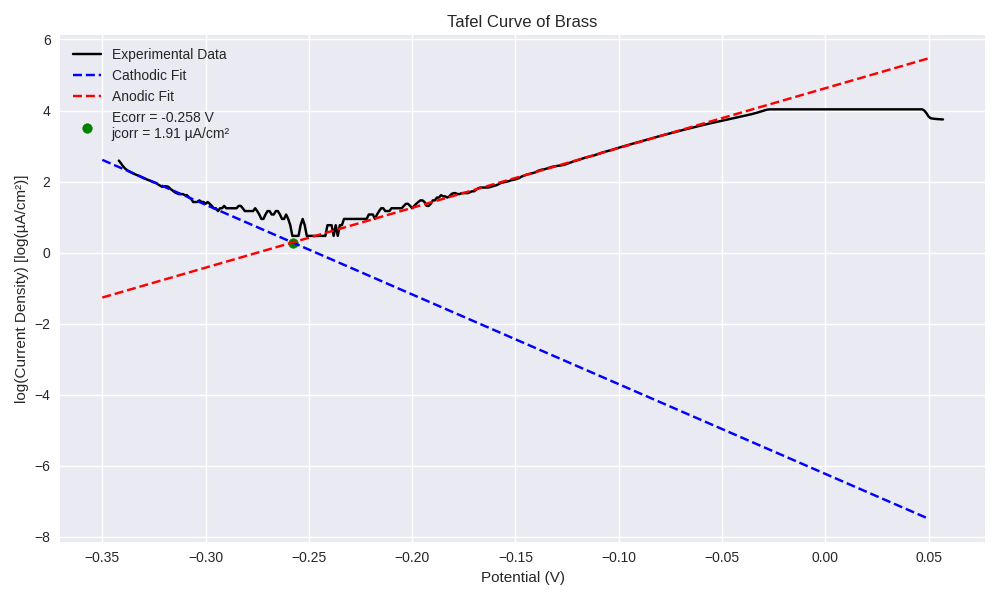
\includegraphics[width=0.7\linewidth]{Figures/TAFEL-BRASS.png}
    \caption{Tafel curve for brass electrode.}
    \label{fig:tafel_brass}
\end{figure}

\vspace{0.2cm}
\subsubsection*{3. Steel Electrode Results}

The steel electrode exhibited higher electrochemical activity. The corrosion parameters were extracted similarly:

\begin{itemize}
    \item \textbf{Corrosion potential:} \( E_{\text{corr}} = -0.388 \) V
    \item \textbf{Corrosion current density:} \( j_{\text{corr}} = 8.87 \times 10^{-5} \) A/cm\(^2\)
    \item \textbf{Anodic fit:} \( \log(j) = 13.650 \cdot E + 1.357 \)
    \item \textbf{Cathodic fit:} \( \log(j) = -5.696 \cdot E - 6.288 \)
\end{itemize}

\begin{figure}[ht!]
    \centering
    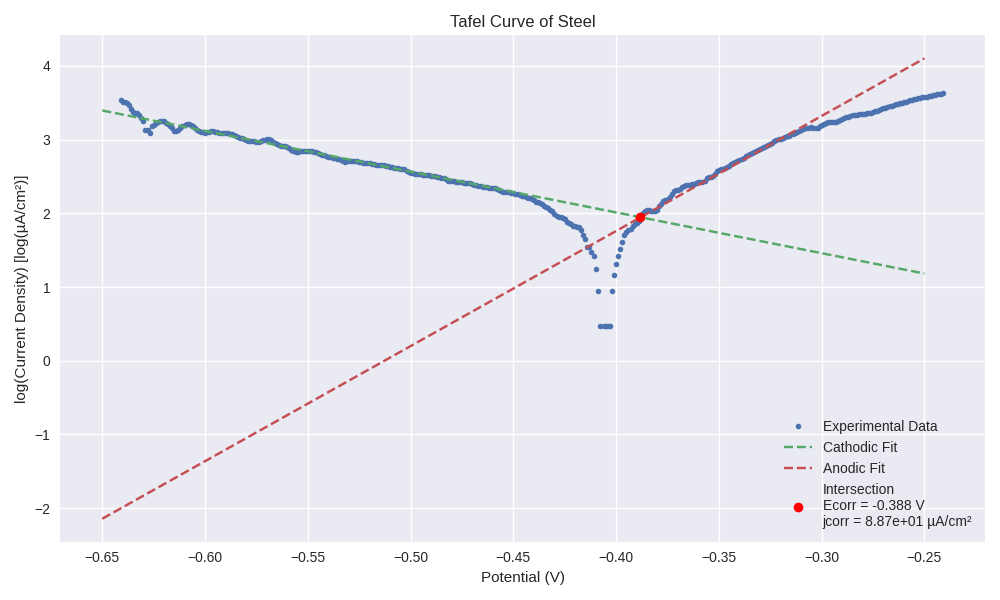
\includegraphics[width=0.7\linewidth]{Figures/TAFEL-STEEL.png}
    \caption{Tafel curve for steel electrode.}
    \label{fig:tafel_steel}
\end{figure}

\vspace{0.2cm}
\subsubsection*{4. Corrosion Penetration Rate (CPR) Calculation}

The CPR was calculated using the empirical formula:

\begin{equation}
\text{CPR} = \frac{0.13 \cdot j_{\text{corr}} \cdot \text{EW}}{\rho}
\end{equation}

Where:
\begin{itemize}
    \item CPR: Corrosion rate (mm/year)
    \item \( j_{\text{corr}} \): Corrosion current density (A/cm\(^2\))
    \item EW: Equivalent weight (g)
    \item \( \rho \): Density (g/cm\(^3\))
\end{itemize}

\vspace{0.2cm}
\textbf{Brass Parameters:}

Table~\ref{tab:cpr_brass} summarizes the main electrochemical parameters obtained for 
the brass electrode. These values were used to calculate the corrosion penetration rate (CPR).

\begin{table}[h!]
\centering
\caption{CPR calculation for brass}
\label{tab:cpr_brass}
\begin{tabular}{|c|c|}
\hline
Parameter & Value \\
\hline
\( j_{\text{corr}} \) & \( 5.40 \times 10^{-6} \) A/cm\(^2\) \\
EW & 50.42 g \\
\( \rho \) & 8.52 g/cm\(^3\) \\
CPR & \( 4.17 \times 10^{-5} \) mm/year \\
\hline
\end{tabular}
\end{table}

\vspace{0.2cm}
\textbf{Steel Parameters:}

Similarly, Table~\ref{tab:cpr_steel} presents the parameters obtained for the steel electrode, 
which show a higher corrosion current density and consequently a higher CPR compared to brass.

\begin{table}[h!]
\centering
\caption{CPR calculation for steel}
\label{tab:cpr_steel}
\begin{tabular}{|c|c|}
\hline
Parameter & Value \\
\hline
\( j_{\text{corr}} \) & \( 8.87 \times 10^{-5} \) A/cm\(^2\) \\
EW & 55.845 g \\
\( \rho \) & 7.85 g/cm\(^3\) \\
CPR & \( 8.23 \times 10^{-4} \) mm/year \\
\hline
\end{tabular}
\end{table}


\vspace{0.2cm}
\subsubsection*{5. Discussion of Results}

The steel electrode exhibited a significantly higher corrosion current density and CPR compared to brass, indicating lower corrosion resistance under the same conditions. The brass electrode showed a flatter Tafel slope and lower \( j_{\text{corr}} \), suggesting more stable electrochemical behavior. These results align with the expected performance of brass in mildly aggressive environments.

The corrosion experiments were conducted in a controlled electrochemical cell using a 0.5 M hydrochloric acid (HCl) solution as the corrosive medium. The presence of chloride ions (\( \text{Cl}^- \)) accelerates the breakdown of passive layers on metal surfaces, promoting localized corrosion and pitting.

The potentiodynamic scans revealed distinct corrosion behaviors:
\begin{itemize}
    \item \textbf{Steel} exhibited a higher corrosion current density and a more negative corrosion potential, indicating greater susceptibility to acid attack.
    \item \textbf{Brass} showed lower current densities and a more stable potential, suggesting better resistance in chloride-rich environments.
\end{itemize}

These differences can be attributed to the alloy composition and surface reactivity. Brass, being a copper-zinc alloy, benefits from the formation of protective oxides and its lower standard electrode potential. Steel, composed primarily of iron, readily oxidizes in acidic media, forming soluble iron ions and unstable corrosion products.

\vspace{0.2cm}
\textbf{Limitations and Considerations:}
\begin{itemize}
    \item The corrosion rates calculated are specific to the 0.5 M HCl medium and may differ significantly in neutral or alkaline environments.
    \item The extrapolation of Tafel lines assumes ideal linearity, which may not fully capture complex surface phenomena such as passivation or film formation.
    \item The reference electrode potential must be corrected if comparing results to literature values based on other reference systems (e.g., NHE).
\end{itemize}

% Conclusion
\section{Conclusion}

Electrochemical analysis using Tafel curves in a 0.5 M HCl medium demonstrated that brass possesses significantly higher corrosion resistance than steel. This is evidenced by its significantly lower corrosion current density $(5.40 * 10^{-6} A/cm^2)$ compared to that of steel $(8.87 * 10^{-5} A/cm^2)$. The superiority of brass is confirmed by calculating the Corrosion Penetration Rate (CPR), which was $4.17 * 10^{-5} mm/year$ for brass, a much lower value than the CPR of steel $(8.23 * 10^{-4} mm/year)$. This practical metric indicates a much slower annual thickness loss. Additionally, the corrosion potential $(E_{corr})$ of brass (-0.258 V) was less negative than that of steel (-0.388 V), reflecting a lower thermodynamic tendency to undergo oxidation. Therefore, if a material needs to be exposed to an acidic environment, brass is much more efficient than steel due to its corrosion resistance.


\section{Questions and Problems}

\textbf{1. What are \( E_{\text{corr}} \), potential resistance, \( j_{\text{corr}} \), and CPR of both metals in the different working solutions?}

\begin{table}[h!]
\centering
\caption{Electrochemical data and CPR calculation for brass}
\label{tab:brass_parameters}
\begin{tabular}{|c|c|}
\hline
Parameter & Value \\
\hline
\( E_{\text{corr}} \) & \( -0.258 \) V \\
Potential Resistance & \( 1.36 \times 10^4 \) \( \Omega\cdot\text{cm}^2 \) \\
\( j_{\text{corr}} \) & \( 5.40 \times 10^{-6} \) A/cm\(^2\) \\
CPR & \( 4.17 \times 10^{-5} \) mm/year \\
\hline
\end{tabular}
\end{table}

\begin{table}[h!]
\centering
\caption{Electrochemical data and CPR calculation for steel}
\label{tab:steel_parameters}
\begin{tabular}{|c|c|}
\hline
Parameter & Value \\
\hline
\( E_{\text{corr}} \) & \( -0.388 \) V \\
Potential Resistance & \( 2.67 \times 10^2 \) \( \Omega\cdot\text{cm}^2 \) \\
\( j_{\text{corr}} \) & \( 8.87 \times 10^{-5} \) A/cm\(^2\) \\
CPR & \( 8.23 \times 10^{-4} \) mm/year \\
\hline
\end{tabular}
\end{table}

\vspace{0.5cm}

\textbf{2. Identify the different regions in the potentiodynamic polarization plots.}


The polarization curves can be divided into cathodic, anodic, and corrosion regions. 
The intersection of the anodic and cathodic branches defines the corrosion potential 
(\(E_{\text{corr}}\)) and the corrosion current density (\(j_{\text{corr}}\)), which are 
used to estimate the corrosion rate. Figures~\ref{fig:tafel_brass} and~\ref{fig:tafel_steel} 
show these regions for brass and steel.

\begin{figure}[ht!]
    \centering
    \begin{subfigure}{0.45\textwidth}
        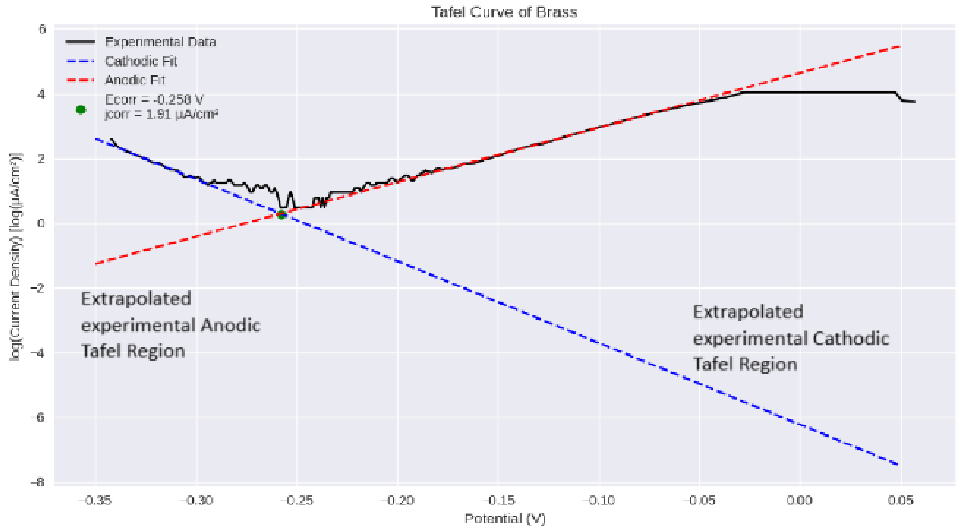
\includegraphics[width=\linewidth]{Figures/Tafel Brass.png}
        \caption{Brass Tafel plot}
        \label{fig:tafel_brass}
    \end{subfigure}
    \hfill
    \begin{subfigure}{0.45\textwidth}
        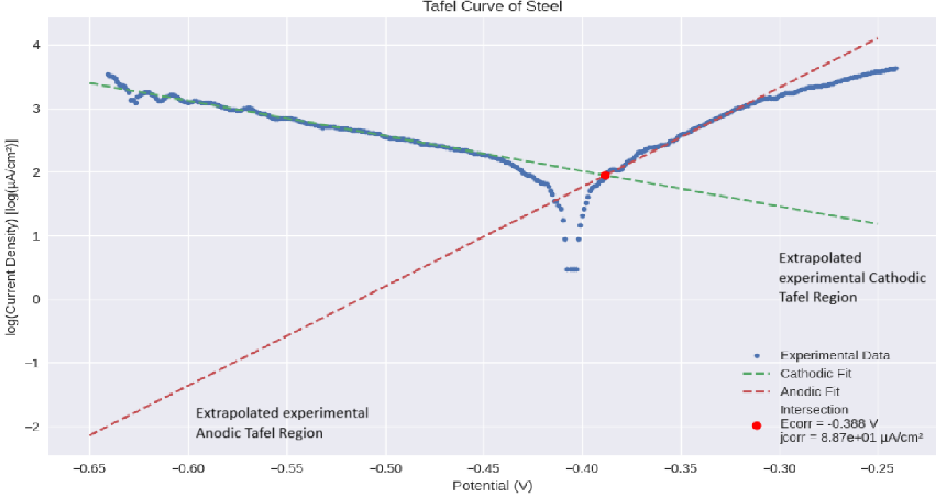
\includegraphics[width=\linewidth]{Figures/Tafel Steel.png}
        \caption{Steel Tafel plot}
        \label{fig:tafel_steel}
    \end{subfigure}
    \caption{Potentiodynamic polarization plots showing anodic, cathodic, and corrosion regions.}
\end{figure}

\vspace{0.5cm}

\textbf{3. Comparison with classmate's results}


\vspace{0.2cm}
\begin{table}[h!]
\centering
\caption{Comparison of electrochemical corrosion results between groups}
\label{tab:cpr_groups}
\begin{tabular}{|c|c|c|c|}
\hline
Group & \( E_{\text{corr}} \) [V] & \( j_{\text{corr}} \) [A/cm\(^2\)] & CPR [mm/year] \\
\hline
\textbf{JJD}  & \(-0.258\) & \( 5.40 \times 10^{-6} \) & \( 4.17 \times 10^{-5} \) \\
\hline
\textbf{GMS}  & \(-0.258\) & \( 1.6217 \times 10^{-6} \) & \( 0.11099 \) \\
\hline
\textbf{RNJM} & \(-0.186\) & \( 9.2204 \times 10^{-6} \) & \( 0.63106 \) \\
\hline
\end{tabular}
\end{table}

Comparison of the electrochemical corrosion results between the three groups reveals significant variations in corrosion kinetics (rate). The JJD and GMS groups shared the same Corrosion Potential ($E_{corr}$) of $-0.258 \text{ V}$, indicating an identical thermodynamic tendency to corrode, which is more negative than that of the RNJM group ($-0.186 \text{ V}$). However, the Corrosion Penetration Rate (CPR), which is the practical rate metric, was drastically different. The RNJM group exhibited the highest corrosion rate with an $i_{corr}$ of $9.2204 \mu\text{A}/\text{cm}^2$ and a CPR of $0.63106 \text{ mm/year}$. At the other extreme, the JJD group showed the best corrosion resistance with the lowest CPR of only $4.17 \times 10^{-5} \text{ mm/year}$, despite its more negative potential.
The large dispersion that exists between the recorded data could be due to the limitations of the equipment used, in addition to the preparation of the sample among other systematic or human errors.



\vspace{0.5cm}

\textbf{4. Comparison with literature values}

Experimental studies on steel corrosion in 0.5 M HCl report \( j_{\text{corr}} \) values typically ranging from \( 10^{-5} \) to \( 10^{-3} \) A/cm\(^2\), depending on steel type, surface condition, temperature, and inhibitor presence. According to Laamari et al.~\cite{laamari_2011_corrosion}, this range is consistent with the measured value for steel (\( 8.87 \times 10^{-5} \) A/cm\(^2\)), confirming its plausibility~\cite{loveday_electrochemical}.

For brass, the measured \( j_{\text{corr}} = 5.4 \times 10^{-6} \) A/cm\(^2\) indicates low corrosivity. Literature reports, such as those by Radovanović et al.~\cite{radovanovi_2019_electrochemical}, show that brass corrosion in HCl is highly sensitive to time, composition, and experimental setup. Differences between literature and experimental results may stem from alloy composition, surface roughness, or environmental factors.

\vspace{0.5cm}

\textbf{5. Would you expect iron to corrode in high-purity water? Why or why not?}

In high-purity water, iron exhibits a very low corrosion rate due to minimal ionic conductivity and the formation of passive oxide/hydroxide films that inhibit anodic dissolution. Additionally, the absence of dissolved oxygen suppresses cathodic reactions, resulting in negligible corrosion. However, trace amounts of oxygen or salts can disrupt passivation and significantly accelerate corrosion.

\vspace{0.5cm}

\textbf{6. Electrochemical behavior of magnesium in different solutions}

\textbf{A) Write the possible oxidation and reduction half-reactions for magnesium in the following media:}

\vspace{0.3cm}
\textbf{(i) HCl solution}



\[
\text{Overall: } \mathrm{Mg}_{(s)} + 2\mathrm{HCl}_{(aq)} \rightarrow \mathrm{Mg}^{2+}_{(aq)} + 2\mathrm{Cl}^{-}_{(aq)} + \mathrm{H}_2\mathrm{(g)}
\]




\[
\text{Oxidation: } \mathrm{Mg}_{(s)} \rightarrow \mathrm{Mg}^{2+}_{(aq)} + 2e^-
\]




\[
\text{Reduction: } 2\mathrm{H}^{+}_{(aq)} + 2e^- \rightarrow \mathrm{H}_2\mathrm{(g)}
\]



\vspace{0.3cm}
\textbf{(ii) HCl solution with dissolved oxygen}



\[
\text{Overall: } 2\mathrm{Mg}_{(s)} + \mathrm{O}_2\mathrm{(g)} + 2\mathrm{H}_2\mathrm{O}_{(l)} \rightarrow 2\mathrm{Mg}^{2+}_{(aq)} + 4\mathrm{OH}^{-}_{(aq)}
\]




\[
\text{Oxidation: } 2\mathrm{Mg}_{(s)} \rightarrow 2\mathrm{Mg}^{2+}_{(aq)} + 4e^-
\]




\[
\text{Reduction: } \mathrm{O}_2\mathrm{(g)} + 2\mathrm{H}_2\mathrm{O}_{(l)} + 4e^- \rightarrow 4\mathrm{OH}^{-}_{(aq)}
\]



\vspace{0.3cm}
\textbf{(iii) HCl solution with dissolved oxygen and Fe\(^{2+}\) ions}



\[
\text{Overall: } \mathrm{Mg}_{(s)} + \frac{1}{2}\mathrm{O}_2\mathrm{(g)} + 2\mathrm{H}_2\mathrm{O}_{(l)} + \mathrm{Fe}^{2+}_{(aq)} \rightarrow \mathrm{Mg}^{2+}_{(aq)} + 4\mathrm{OH}^{-}_{(aq)} + \mathrm{Fe}_{(s)}
\]




\[
\text{Oxidation: } \mathrm{Mg}_{(s)} \rightarrow \mathrm{Mg}^{2+}_{(aq)} + 2e^-
\]




\[
\text{Reduction 1: } \mathrm{Fe}^{2+}_{(aq)} + 2e^- \rightarrow \mathrm{Fe}_{(s)}
\]




\[
\text{Reduction 2: } \frac{1}{2}\mathrm{O}_2\mathrm{(g)} + 2\mathrm{H}_2\mathrm{O}_{(l)} + 2e^- \rightarrow 4\mathrm{OH}^{-}_{(aq)}
\]



\vspace{0.5cm}

\textbf{B) In which solution would magnesium oxidize most rapidly? Why?}

Magnesium is expected to oxidize most rapidly in the HCl solution containing both dissolved oxygen and Fe\(^{2+}\) ions. These species act as strong oxidizing agents, enhancing cathodic reactions and accelerating the overall corrosion rate. The presence of multiple electron acceptors increases the electrochemical driving force for magnesium dissolution.





\printbibliography


\end{document}
